\documentclass{article}
\usepackage{tikz}
\usepackage{circuitikz}
\usepackage{verbatim}
\usepackage{pst-circ}

\begin{comment}
:Title: Circuit RLC

\end{comment}

\begin{document}


\begin{circuitikz} [ scale =1.1, american]
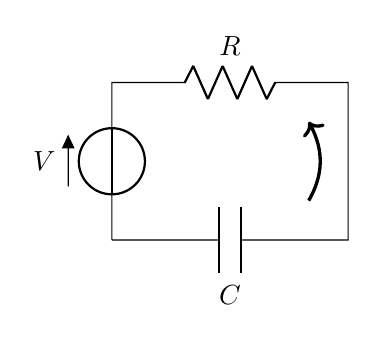
\begin{tikzpicture}
	\newcommand*{\equal}{=}
	\draw  (0,0)
		to[V,v=$V$] (0,2)		% sV,v=   (t)\equal cost
							% R_1\equal 20\,\Omega
		to[R=$R  $ ] (3,2) 		% \equal .05\,F
		to [short] (3, 0)
		to[C=$C  $ ] (0, 0);
	%	\draw [very thick, ->, blue]  (3,1)--(3,1.5);
	 \draw [very thick, ->] (2.5, .5) to[bend right] (2.5, 1.5);

%	to[ospst] (0,0);

%	\draw  (0,0)
%		to[V,v=$U_q$] (0,2) % The voltage source
%		to[short] (2,2)
%		to[R=$R_1$] (2,0)  % The resistor
%		to[short] (0,0);

%	\draw (2,2)
%		to[short] (4,2)
%		to[L=$L_1$] (4,0)
%		to[short] (2,0);
%	\draw (4,2)
%		to[short] (6,2)
%		to[C=$C_1$] (6,0)
%		to[short] (4,0);

\end{tikzpicture} 
\end{circuitikz}
\end{document}